\chapter{Arquitetura}
\label{chap:arquitetura}

\begin{introduction}
Este capítulo detalha de que forma os objetivos influenciaram a arquitetura, apresenta a arquitetura lógica e descreve as tecnologias escolhidas para a concretizar.
\end{introduction}

\section{Requisitos e o seu Impacto na Arquitetura}

\subsection{Objetivos e Requisitos}

Como descrito na Secção~\ref{sec:objectives}, os objetivos principais para este trabalho são:
\begin{itemize}
    \item Demonstrar a exequibilidade do paradigma de \textit{streaming}
    \item Integrar fontes de dados fundamentadas na literatura
    \item Ilustrar a monitorização em tempo real
    \item Projetar uma arquitetura modular
\end{itemize}

Tendo em conta estes objetivos para este trabalho, decidi estabelecer os seguintes requisitos para o sistema:
\begin{itemize}
    \item \textbf{Suporte para recolha de dados de múltiplos utilizadores em simultâneo:} de modo a cumprir com o cenário estabelecido, o sistema tem de ser projetado para receber dados de vários clientes em simultâneo
    \item \textbf{Suporte para o uso de múltiplos periféricos e dispositivos \textit{wearable off-the-shelf}}: o sistema tem de ser capaz de ingerir dados de periféricos (teclado e câmara) e de dispositivos \textit{wearable off-the-shelf} (\textit{smartwatch wearOS}) para um mesmo utilizador.
    \item \textbf{Suporte para ferramentas de visualização:} de modo a permitir a visualização dos dados (em tempo real ou históricos), o sistema tem de ser capaz de integrar \textit{software} de visualização
    \item \textbf{Suporte à adição de sensores:} devido à diversidade de casos de uso dentro do cenário indicado, o sistema tem de ser capaz de permitir que novos \textit{wearables} ou periféricos sejam adicionados e que novas métricas sejam extraídas com base nas necessidades específicas.
\end{itemize}

\subsection{Impacto dos Requisitos no Sistema}

Em primeiro lugar, a necessidade de suportar a recolha de múltiplos utilizadores, bem como a escolha do \textit{streaming} como paradigma levou à separação do sistema em dois blocos lógicos: o subsistema do cliente presente em cada computador e um subsistema remoto partilhado para onde os clientes enviam os dados para serem processados e armazenados.
Contudo, a necessidade de suportar várias fontes de dados, especialmente tendo em conta que alguns \textit{wearables} não conseguem comunicar diretamente com o servidor, leva à transferência da responsabilidade de coordenação dos vários sensores de cada utilizador para o subsistema do cliente, servindo assim como agregador (ou \textit{buffer} local dos dados).
Esta separação de responsabilidades facilita também o cumprimento do requisito do suporte à adição de sensores, pois permite que o servidor seja geralmente agnóstico à origem dos dados e as suas características, isolando assim o esforço de modificação ao subsistema do cliente.

Em segundo lugar, a necessidade de visualização, favorece o armazenamento dos dados numa base de dados (ou um sistema de persistência equivalente), visto que assim é possível não só analisar o estado atual, mas também consultar dados históricos (permitindo, por exemplo, diferenciar entre um momento pontual de cansaço e uma tendência regular provocada por \textit{burnout}).
Contudo, devido à natureza heterogénea dos dados (bem como a necessidade de agrupar os dados por tipo de sensor), torna-se necessário armazenar os dados em estruturas de dados diferentes (tendo cada estrutura um \textit{schema} diferente) o que poderá ser assegurado ao estabelecer um esquema de roteamento automático, o que pode ser realizado utilizando diferentes tópicos com um prefixo comum ou através da injeção do tipo de sensor no \textit{payload} enviado.

Finalmente, como um dos objetivos do trabalho é utilizar especificamente o paradigma de \textit{streaming} para a recolha destes dados, para assim demonstrar a sua exequibilidade neste cenário, não só torna mais relevante a escolha ponderada das tecnologias a utilizar, mas também favorece a resolução de problemas explorando soluções de \textit{streaming} existentes, em vez de recorrer a código escrito de raiz. 

\section{Arquitetura Lógica}

O diagrama de componentes presente na Figura~\ref{fig:sys_arq_logic} apresenta a estrutura a alto nível do sistema, podendo ser dividido em dois subsistemas:
\begin{itemize}
    \item \textbf{Subsistema Local (Cliente):} Este subsistema é executado no computador do utilizador e pretende recolher e agregar dados de sensores. Para além dos sensores (que podem ser parte do próprio computador ou serem externos a este), este subsistema é composto por uma \textbf{Aplicação} responsável pelo controlo dos sensores e por um \textbf{\textit{Broker} Local}, que serve como intermediário para a comunicação com sensores externos e como \textit{buffer} no envio de dados para o servidor.
    \item \textbf{Subsistema Remoto (Servidor):} Este subsistema é executado num servidor remoto e visa a recolha, armazenamento e disponibilização dos dados de forma contínua. Este subsistema é composto por uma \textbf{\textit{Pipeline} para recolha de dados} capaz de os processar em \textit{streaming} contínuo, uma \textbf{Base de dados} para os armazenar e finalmente uma \textbf{API} para gerir a consulta de dados.
\end{itemize}

\begin{figure}
    \centering
    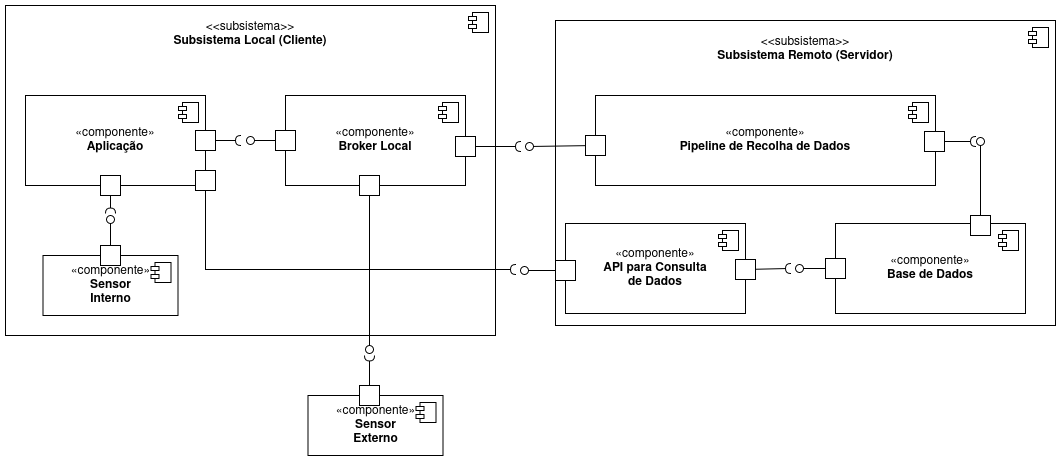
\includegraphics[width=\linewidth]{figs/logical_arquitecture.png}
    \caption{Diagrama de componentes do sistema}
    \label{fig:sys_arq_logic}
\end{figure}

\section{Tecnologias Escolhidas}

Após o estabelecimento dos blocos lógicos e da escolha dos sensores a utilizar para demonstrar as capacidades do sistema (câmara, teclado e \ac{BPM} via \textit{smartwatch WearOS}), prossegui à escolha das ferramentas e tecnologias para implementar cada um dos blocos lógicos.

Para a aplicação, decidi fazer uma interface gráfica em \textbf{Python}, utilizando uma estrutura baseada num registo de \textit{plugins}, não só pela versatilidade da linguagem, mas também por considerar ser uma das linguagens de programação mais fáceis de aprender, diminuindo assim a barreira de acesso para investigadores com pouco conhecimento em programação.

Para o \textit{broker} local, decidi utilizar o \textbf{Mosquitto}, que desempenha duas funções: atua como \textit{buffer} local em caso de falha de rede e serve como intermediário para comunicar com o \textit{smartwatch}, pois apesar de ter sido preferível o uso do protocolo \ac{BLE}, alguns dispositivos (como o Xiaomi Watch 2 que utilizei neste trabalho), optam por utilizar uma interface proprietária~\cite{blexiaomi}, dificultando assim a comunicação direta entre aplicações.

Para o \textit{smartwatch}, optei por desenvolver uma aplicação em Kotlin para \textit{WearOS} para facilitar a comunicação com o computador (sendo que escolhi Kotlin em particular por ser a linguagem oficial para desenvolvimento em \textit{WearOS}).

Para a \textit{pipeline} de ingestão de dados, decidi utilizar as três seguintes tecnologias:
\begin{itemize}
    \item \textbf{Kafka:} escolhi o Kafka como base da \textit{pipeline} por oferecer um modelo de \textit{streaming} robusto e com melhor resiliência a falhas do que o \ac{MQTT}.
    \item \textbf{Kafka Connect:} para a ingestão dos dados no Kafka e a sua inserção na base de dados, decidi utilizar o Kafka Connect em vez de uma implementação própria, por já possuir mecanismos para lidar com falhas transitórias e por possuir uma grande variedade de conectores prontos a utilizar (reduzindo assim o esforço para troca de componentes ou integração com bases de dados pré-existentes).
    \item \textbf{Mosquitto:} finalmente, como o estabelecimento de um conector para cada cliente apresenta problemas de escalabilidade e possivelmente de segurança (visto que algumas \textit{firewalls} bloqueiam conexões \textit{inbound}), decidi também utilizar um segundo \textit{broker \ac{MQTT}} como ponto principal de acesso para ingestão (sendo que a movimentação de dados entre o \textit{broker} local e o \textit{broker} remoto é realizado de forma automática pelo próprio Mosquitto).
\end{itemize}

Para a base de dados, visto que os dados a armazenar são medições de sensores (que são dados naturalmente indexados por tempo), optei por uma base de dados \textit{Time Series}. Em particular, escolhi o InfluxDB pela sua popularidade e boa documentação (características particularmente úteis para um projeto individual com prazo limitado).

Finalmente, por questões de segurança, decidi utilizar uma API \ac{REST} escrita em Python (por permitir criar um servidor simples com um mínimo de código \textit{boilerplate}) para servir como intermediário no acesso aos dados por parte do cliente, reduzindo assim o risco de injeção de \textit{queries}.

De modo a ilustrar melhor a estrutura do sistema após a escolha das tecnologias, eu desenhei o diagrama de \textit{deployment} presente na Figura~\ref{fig:sys_arq_deployment}.

\begin{figure}
    \centering
    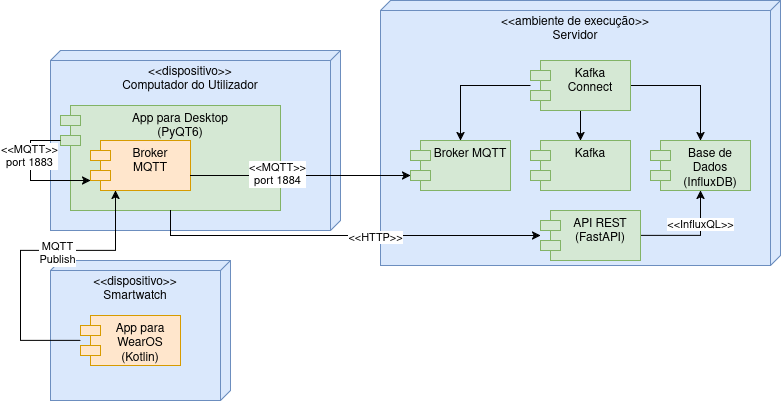
\includegraphics[width=\linewidth]{figs/deployment_arquitecture.png}
    \caption{Diagrama de \textit{deployment} do sistema}
    \label{fig:sys_arq_deployment}
\end{figure}

\section{Fluxo de Dados}

De modo a ilustrar como estes componentes comunicam entre si, a Figura~\ref{fig:end2end} mapeia o fluxo de dados \textit{end-to-end}, utilizando como exemplo os dados faciais obtidos via \textit{webcam}:

\begin{itemize}
    \item \textbf{Captura e ingestão} (passos 1 a 3): O \textit{plugin} da \textit{webcam} presente na aplicação \textit{desktop} captura uma \textit{frame} e extrai as \textit{features} faciais. Estas \textit{features} são convertidas em métricas (de modo a reduzir o volume de dados a enviar) e enviadas para o \textit{broker} Mosquitto local.
    \item \textbf{Redirecionamento} (passo 4) Os dados presentes no broker local (em tópicos com o prefixo \texttt{sensors/}) são redirecionados para um \textit{broker} remoto automaticamente.
    \item \textbf{Transporte:} (passos 5 a 7) Após a chegada de novos dados ao \textit{broker}, o conector \textit{source} do Kafka Connect recolhe estes dados e insere-os no Kafka (que possui melhor resiliência que o Mosquitto, permitindo ingestão assíncrona).
    \item \textbf{Armazenamento} (passos 8 a 10): Após a inserção no Kafka, um segundo conector \textit{sink} de Kafka Connect consome as mensagens e armazena-as na base de dados.
    \item \textbf{Acesso e visualização} (secção ``Visualização de dados''): Após o armazenamento dos dados, estes são acedidos via API REST pela app \textit{desktop} a cada segundo para gerar uma visualização dos dados.
\end{itemize}

\begin{figure}
    \centering
    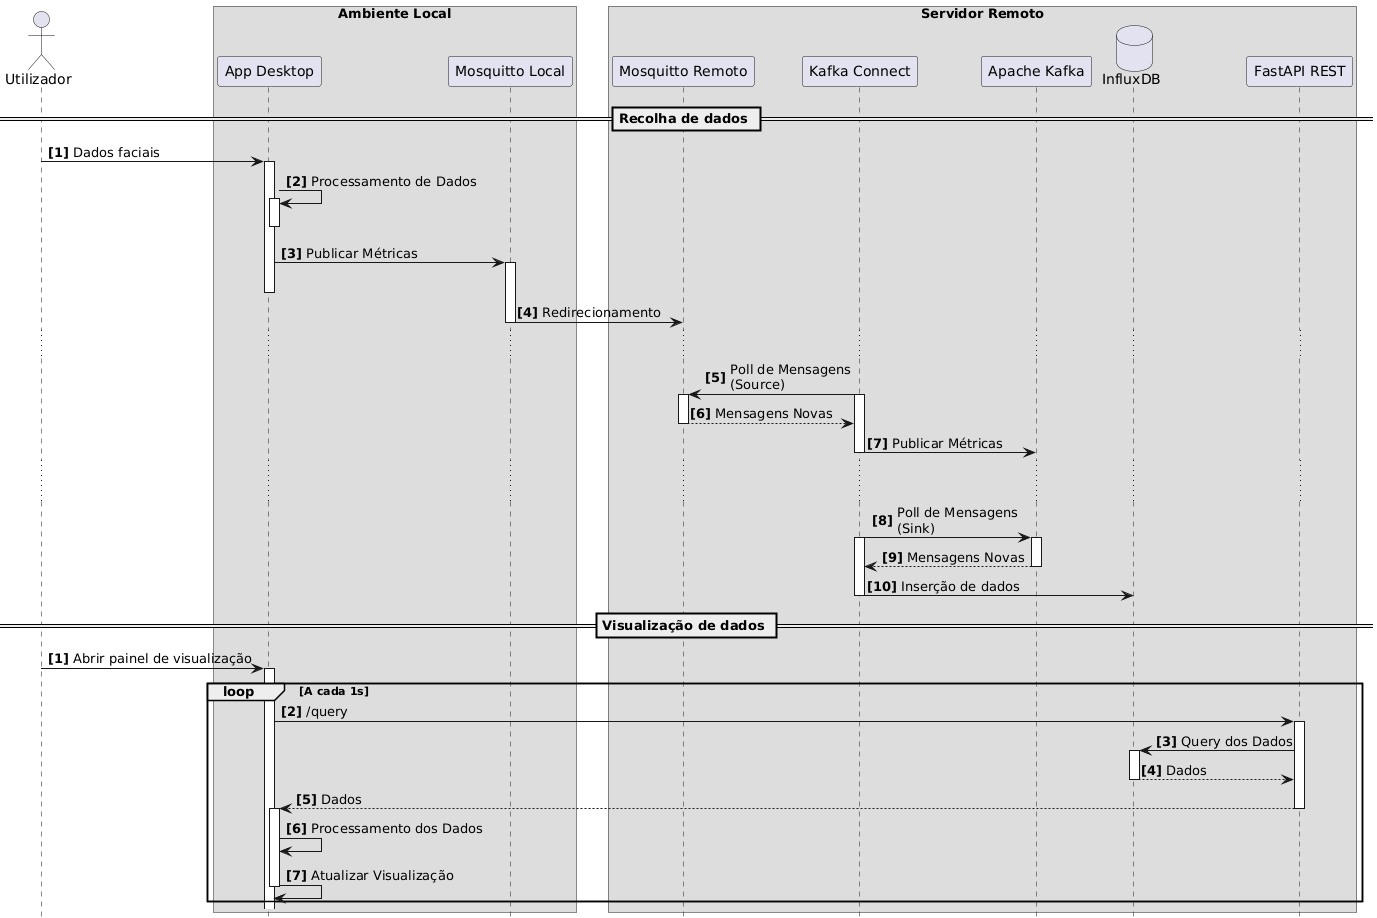
\includegraphics[width=\linewidth]{figs/end2end.png}
    \caption{Fluxo de dados \textit{end-to-end}}
    \label{fig:end2end}
\end{figure}